\documentclass[14pt]{extbook}
\usepackage{multicol, enumerate, enumitem, hyperref, color, soul, setspace, parskip, fancyhdr} %General Packages
\usepackage{amssymb, amsthm, amsmath, latexsym, units, mathtools} %Math Packages
\everymath{\displaystyle} %All math in Display Style
% Packages with additional options
\usepackage[headsep=0.5cm,headheight=12pt, left=1 in,right= 1 in,top= 1 in,bottom= 1 in]{geometry}
\usepackage[usenames,dvipsnames]{xcolor}
\usepackage{dashrule}  % Package to use the command below to create lines between items
\newcommand{\litem}[1]{\item#1\hspace*{-1cm}\rule{\textwidth}{0.4pt}}
\pagestyle{fancy}
\lhead{Progress Quiz 5}
\chead{}
\rhead{Version C}
\lfoot{8497-6012}
\cfoot{}
\rfoot{Summer C 2021}
\begin{document}

\begin{enumerate}
\litem{
Determine the vertical asymptotes and holes in the rational function below.\[ f(x) = \frac{8x^{3} +26 x^{2} -33 x -36}{16x^{2} -8 x -15} \]\begin{enumerate}[label=\Alph*.]
\item \( \text{Vertical Asymptotes of } x = 1.25 \text{ and } x = -0.75 \text{ with no holes.} \)
\item \( \text{Vertical Asymptotes of } x = 1.25 \text{ and } x = 1.5 \text{ with a hole at } x = -0.75 \)
\item \( \text{Vertical Asymptote of } x = 0.5 \text{ and hole at } x = -0.75 \)
\item \( \text{Holes at } x = 1.25 \text{ and } x = -0.75 \text{ with no vertical asymptotes.} \)
\item \( \text{Vertical Asymptote of } x = 1.25 \text{ and hole at } x = -0.75 \)

\end{enumerate} }
\litem{
Determine the vertical asymptotes and holes in the rational function below.\[ f(x) = \frac{12x^{3} +11 x^{2} -45 x -50}{6x^{2} +x -15} \]\begin{enumerate}[label=\Alph*.]
\item \( \text{Holes at } x = 1.5 \text{ and } x = -1.667 \text{ with no vertical asymptotes.} \)
\item \( \text{Vertical Asymptote of } x = 1.5 \text{ and hole at } x = -1.667 \)
\item \( \text{Vertical Asymptotes of } x = 1.5 \text{ and } x = -1.667 \text{ with no holes.} \)
\item \( \text{Vertical Asymptote of } x = 2.0 \text{ and hole at } x = -1.667 \)
\item \( \text{Vertical Asymptotes of } x = 1.5 \text{ and } x = -1.25 \text{ with a hole at } x = -1.667 \)

\end{enumerate} }
\litem{
Determine the vertical asymptotes and holes in the rational function below.\[ f(x) = \frac{12x^{3} +17 x^{2} -14 x -15}{12x^{2} +x -6} \]\begin{enumerate}[label=\Alph*.]
\item \( \text{Vertical Asymptotes of } x = 0.667 \text{ and } x = -0.75 \text{ with no holes.} \)
\item \( \text{Vertical Asymptote of } x = 1.0 \text{ and hole at } x = -0.75 \)
\item \( \text{Vertical Asymptote of } x = 0.667 \text{ and hole at } x = -0.75 \)
\item \( \text{Vertical Asymptotes of } x = 0.667 \text{ and } x = -1.667 \text{ with a hole at } x = -0.75 \)
\item \( \text{Holes at } x = 0.667 \text{ and } x = -0.75 \text{ with no vertical asymptotes.} \)

\end{enumerate} }
\litem{
Determine the vertical asymptotes and holes in the rational function below.\[ f(x) = \frac{8x^{3} +18 x^{2} -15 x -25}{12x^{2} -31 x + 20} \]\begin{enumerate}[label=\Alph*.]
\item \( \text{Vertical Asymptotes of } x = 1.333 \text{ and } x = -2.5 \text{ with a hole at } x = 1.25 \)
\item \( \text{Vertical Asymptotes of } x = 1.333 \text{ and } x = 1.25 \text{ with no holes.} \)
\item \( \text{Holes at } x = 1.333 \text{ and } x = 1.25 \text{ with no vertical asymptotes.} \)
\item \( \text{Vertical Asymptote of } x = 0.667 \text{ and hole at } x = 1.25 \)
\item \( \text{Vertical Asymptote of } x = 1.333 \text{ and hole at } x = 1.25 \)

\end{enumerate} }
\litem{
Determine the horizontal and/or oblique asymptotes in the rational function below.\[ f(x) = \frac{12x^{3} +25 x^{2} -4 x -12}{4x^{2} +23 x + 15} \]\begin{enumerate}[label=\Alph*.]
\item \( \text{Oblique Asymptote of } y = 3x -11. \)
\item \( \text{Horizontal Asymptote of } y = 3.0  \)
\item \( \text{Horizontal Asymptote of } y = 3.0 \text{ and Oblique Asymptote of } y = 3x -11 \)
\item \( \text{Horizontal Asymptote of } y = -5.0 \text{ and Oblique Asymptote of } y = 3x -11 \)
\item \( \text{Horizontal Asymptote at } y = -5.0 \)

\end{enumerate} }
\litem{
Determine the horizontal and/or oblique asymptotes in the rational function below.\[ f(x) = \frac{12x^{3} +83 x^{2} +165 x + 100}{3x^{3} -5 x^{2} -65 x -100} \]\begin{enumerate}[label=\Alph*.]
\item \( \text{Vertical Asymptote of } y = -4  \)
\item \( \text{None of the above} \)
\item \( \text{Horizontal Asymptote of } y = 0  \)
\item \( \text{Horizontal Asymptote of } y = 4.000  \)
\item \( \text{Vertical Asymptote of } y = 5.000  \)

\end{enumerate} }
\litem{
Which of the following functions \textit{could} be the graph below?
\begin{center}
    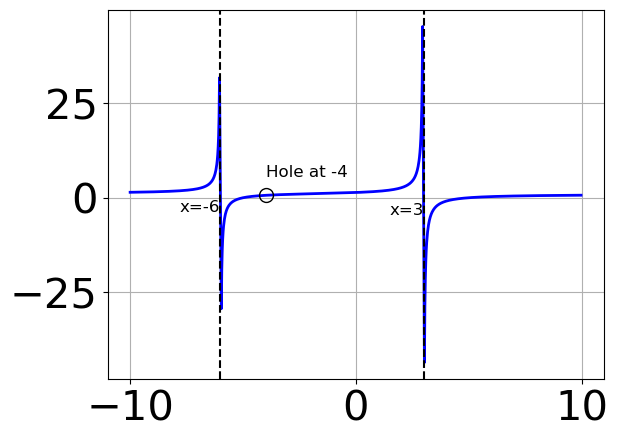
\includegraphics[width=0.5\textwidth]{../Figures/identifyGraphOfRationalFunctionCopyC.png}
\end{center}
\begin{enumerate}[label=\Alph*.]
\item \( f(x)=\frac{x^{3} -5.0 x^{2} -25.0 x + 125.0}{x^{3} -7.0 x^{2} -6.0 x + 72.0} \)
\item \( f(x)=\frac{x^{3} -5.0 x^{2} -25.0 x + 125.0}{x^{3} +7.0 x^{2} -6.0 x -72.0} \)
\item \( f(x)=\frac{x^{3} +4.0 x^{2} -25.0 x -100.0}{x^{3} +7.0 x^{2} -6.0 x -72.0} \)
\item \( f(x)=\frac{x^{3} -4.0 x^{2} -25.0 x + 100.0}{x^{3} -7.0 x^{2} -6.0 x + 72.0} \)
\item \( \text{None of the above are possible equations for the graph.} \)

\end{enumerate} }
\litem{
Determine the horizontal and/or oblique asymptotes in the rational function below.\[ f(x) = \frac{5x^{2} +27 x + 10}{15x^{3} + x^{2} -12 x -4} \]\begin{enumerate}[label=\Alph*.]
\item \( \text{Horizontal Asymptote of } y = 0.333 \text{ and Oblique Asymptote of } y = 3x -16 \)
\item \( \text{Horizontal Asymptote at } y = -5.000 \)
\item \( \text{Horizontal Asymptote of } y = 0 \)
\item \( \text{Oblique Asymptote of } y = 3x -16. \)
\item \( \text{Horizontal Asymptote of } y = 0.333  \)

\end{enumerate} }
\litem{
Which of the following functions \textit{could} be the graph below?
\begin{center}
    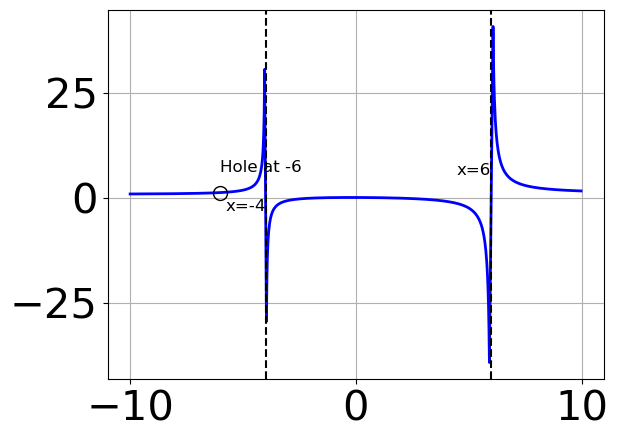
\includegraphics[width=0.5\textwidth]{../Figures/identifyGraphOfRationalFunctionC.png}
\end{center}
\begin{enumerate}[label=\Alph*.]
\item \( f(x)=\frac{x^{3} -2.0 x^{2} -4.0 x + 8.0}{x^{3} -4.0 x^{2} -36.0 x + 144.0} \)
\item \( f(x)=\frac{x^{3} -6.0 x^{2} -4.0 x + 24.0}{x^{3} -4.0 x^{2} -36.0 x + 144.0} \)
\item \( f(x)=\frac{x^{3} +6.0 x^{2} -4.0 x -24.0}{x^{3} +4.0 x^{2} -36.0 x -144.0} \)
\item \( f(x)=\frac{x^{3} +3.0 x^{2} -4.0 x -12.0}{x^{3} +4.0 x^{2} -36.0 x -144.0} \)
\item \( \text{None of the above are possible equations for the graph.} \)

\end{enumerate} }
\litem{
Determine the horizontal and/or oblique asymptotes in the rational function below.\[ f(x) = \frac{4x^{3} -8 x^{2} -25 x + 50}{2x^{2} -x -10} \]\begin{enumerate}[label=\Alph*.]
\item \( \text{Horizontal Asymptote of } y = 2.0  \)
\item \( \text{Horizontal Asymptote of } y = -2.0 \text{ and Oblique Asymptote of } y = 2x -3 \)
\item \( \text{Horizontal Asymptote of } y = 2.0 \text{ and Oblique Asymptote of } y = 2x -3 \)
\item \( \text{Oblique Asymptote of } y = 2x -3. \)
\item \( \text{Horizontal Asymptote at } y = -2.0 \)

\end{enumerate} }
\end{enumerate}

\end{document}